\section{Das Nautische Dreieck}
\kopfrechts{Das nautische Dreieck}
\subsection{Definition des Nautischen Dreiecks}
\index{Himmelskugel}%
Die Himmelskugel ist eine gedachte Kugel, welche die Erde und dessen Beobachter umgibt und als Rechenfläche für Koordinaten in der Astronomie und Geodäsie dient.
\index{Geodäsie}%
Der Zenit ist jener Punkt, der vom Erdmittelpunkt durch denn eigenen Standort an die Himmelskugel verlängert wird.
\index{Zenit}%
Als Gestirne kommen Sterne und Planeten in Frage, zu welchen in diversen Jahrbüchern die für die Navigation nötigen Daten publiziert sind.
\index{Jahrbuch}%
Der Himmelspol ist der Nordpol an die Himmelskugel projiziert.
\index{Himmelspol}%
Das nautische Dreieck hat die Ecken Zenit, Gestirn und Himmelspol, wie man in der Abbildung \ref{naut} sehen kann.
\index{nautisches Dreieck}%
\index{Dreieck, nautisches}%

Ursprünglich ist das nautische Dreieck ein Hilfsmittel der sphärischen
Astronomie um die momentane Position eines Fixsterns oder Planeten
an der Himmelskugel zu bestimmen.

\subsection{Das Bilddreieck}
\begin{figure}
\centering
		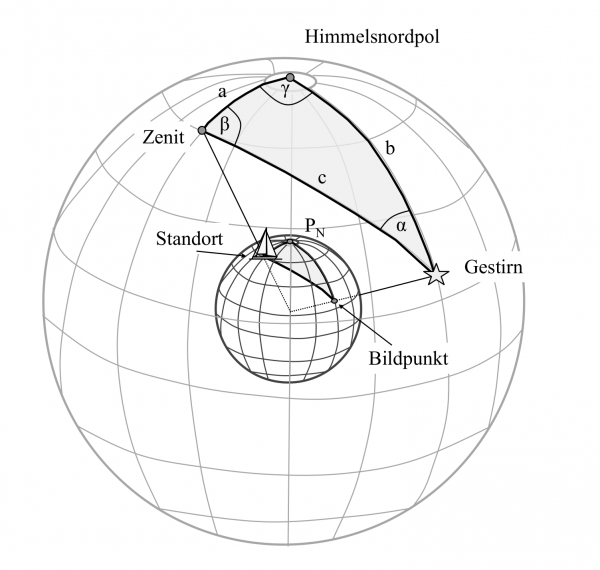
\includegraphics[width=8cm]{papers/nav/bilder/kugel3.png}
		\caption[Nautisches Dreieck]{Nautisches Dreieck}
		\label{naut}
\end{figure}
 Man kann das nautische Dreieck auf die Erdkugel projizieren.
Dieses Dreieck nennt man dann Bilddreieck.
\index{Bilddreieck}%
Als Bildpunkt wird in der astronomischen Navigation der Punkt bezeichnet, an dem eine gedachte Linie vom Mittelpunkt eines beobachteten Gestirns zum Mittelpunkt der Erde die Erdoberfläche schneidet. 
\index{Bildpunkt}%
Die Projektion des nautischen Dreiecks auf die Erdkugel hat die Ecken Nordpol, Standort und Bildpunkt.

\section{Standortbestimmung ohne elektronische Hilfsmittel}
\label{sta}
\kopfrechts{Standortbestimmung ohne elektronische Hilfsmittel}
Um den eigenen Standort herauszufinden, wird in diesem Kapitel die Projektion des nautische Dreiecks auf die Erdkugel zur Hilfe genommen.
Mithilfe eines Sextanten, einem Jahrbuch und der sphärischen Trigonometrie kann man dann die Längen- und Breitengrade des eigenen Standortes bestimmen.
Was ein Sextant und ein Jahrbuch ist, wird im Abschnitt \ref{ephe} erklärt.
\index{Sextant}%
\begin{figure}
\centering
	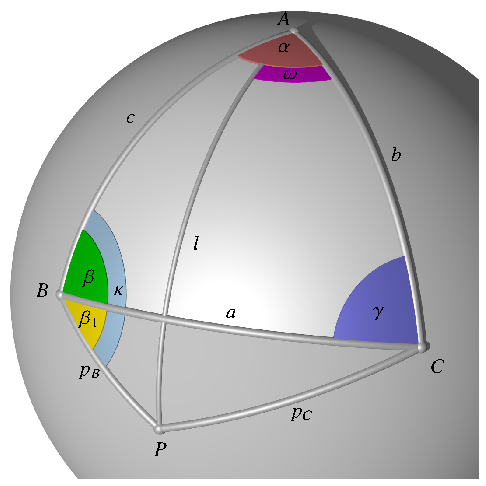
\includegraphics[width=10cm]{papers/nav/images/dreieck3d8.pdf}
	\caption[Dreieck für die Standortbestimmung]{Dreieck für die Standortbestimmung}
	\label{d1}
\end{figure}




\subsection{Ecke $P$ und $A$}
Unser eigener Standort ist der gesuchte Ecke $P$ und die Ecke $A$ ist in unserem Fall der Nordpol.
Der Vorteil an der Idee des nautischen Dreiecks ist, dass eine Ecke immer der Nordpol ist.
Somit ist diese Ecke immer bekannt und nur deswegen sind die Zusammenhänge von Rektaszension, Sternzeit und Deklination so einfach.

\subsection{Ecke $B$ und $C$ - Bildpunkt von $X$ und $Y$}
Für die Standortermittlung benötigt man als weiteren Punkt ein Gestirn
bzw.~seinen Bildpunkt auf der Erdkugel. 
Damit das trigonometrische Rechnen einfacher wird, werden hier zwei Gestirne zur Hilfe genommen.
Es gibt diverse Gestirne, die man nutzen kann wie zum Beispiel die Sonne, der Mond oder die vier Navigationsplaneten Venus, Mars, Jupiter und Saturn.

Die Bildpunkte von den beiden Gestirnen $X$ und $Y$ bilden die beiden Ecken $B$ und $C$ im Dreieck der Abbildung \ref{d1}.
\subsection{Ephemeriden}
\label{ephe}
Zu all diesen Gestirnen gibt es Ephemeridentabellen.
\index{Ephemeriden}%
Diese Tabellen (siehe Abbildung~\ref{nav:fig:eph}) enthalten die
Rektaszensionen und Deklinationen in Abhängigkeit von der Zeit.
\begin{figure}
\centering
	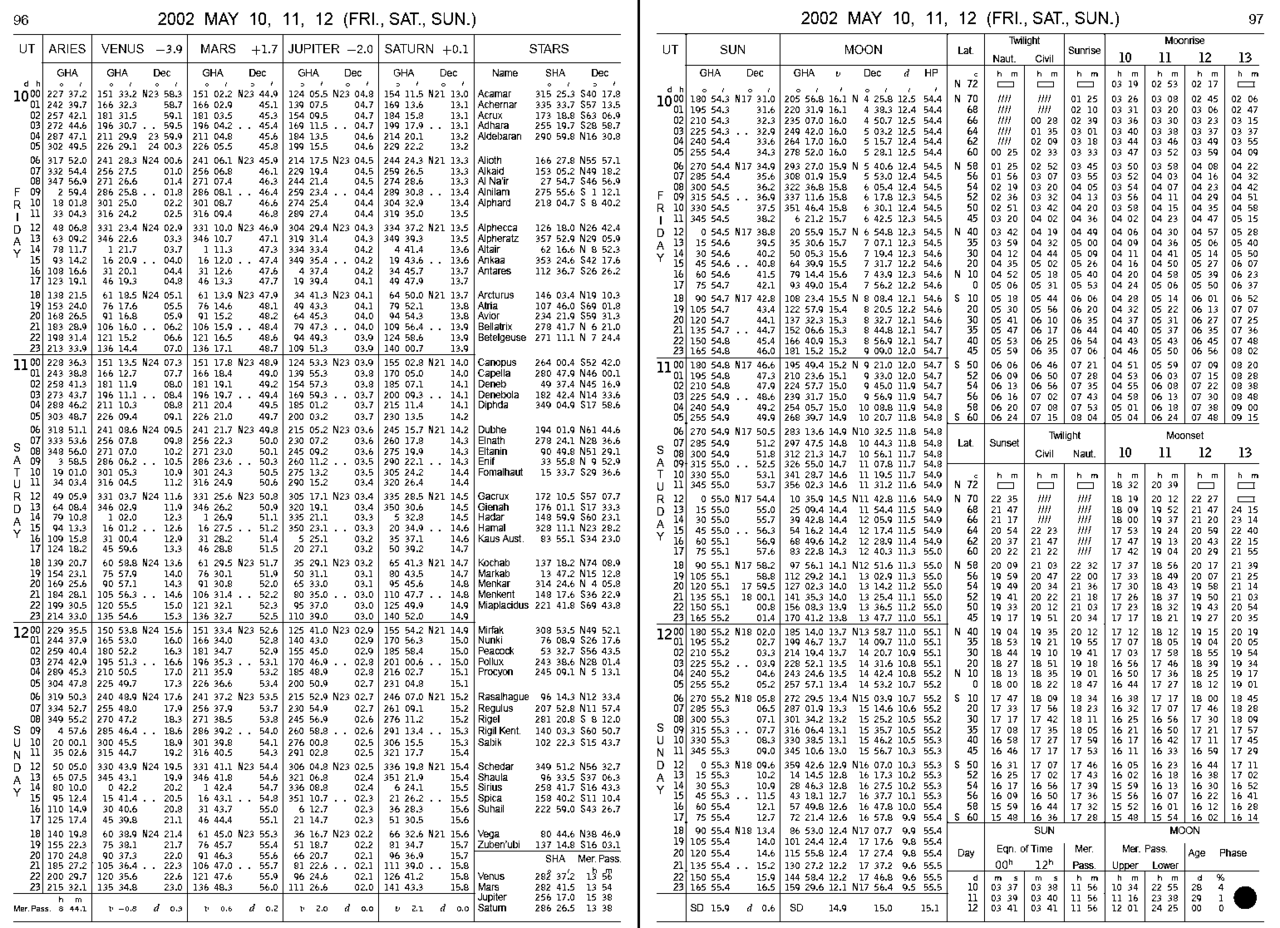
\includegraphics[width=\textwidth]{papers/nav/bilder/ephe.png}
	\caption[Nautical Almanac Mai 2002]{Nautical Almanac Mai 2002}
	\label{nav:fig:eph}
\end{figure}

\subsubsection{Deklination}
\index{Deklination}%
Die Deklination $\delta$ beschreibt den Winkel zwischen dem Himmelsäquator und Gestirn und entspricht dem Breitengrad des Gestirns.

\subsubsection{Rektaszension und Sternzeit}
\index{Rektaszension}%
Die Rektaszension $\alpha$ gibt an, in welchem Winkel das Gestirn
zum Frühlingspunkt, welcher der Nullpunkt auf dem Himmelsäquator
\index{Frühlingspunkt}%
ist, steht und geht vom Koordinatensystem der Himmelskugel aus.

Die Tatsache, dass sich die Himmelskugel  ca.~vier Minuten schneller
um die eigene Achse dreht als die Erdkugel, stellt hier ein kleines
Problem dar.
Die Lösung ist die Sternzeit $\theta$. 
\index{Sternzeit}%
Mit dieser können wir die schnellere Drehung der Himmelskugel ausgleichen.
Die Sternzeit geht vom Frühlungspunkt aus, an welchem die Sonne den Himmelsäquator schneidet und $\theta=0$ ist. 
Für die Standortermittlung auf der Erdkugel ist es am einfachsten, wenn man die Sternzeit von Greenwich berechnet. 
Für die Sternzeit von Greenwich $\theta$ braucht man als erstes das Julianische Datum $T$ vom aktuellen Tag, welches sich leicht nachschlagen lässt.
\index{julianisches Datum}%
Im Anschluss berechnet man die Sternzeit von Greenwich
\[
\theta = 6^h 41^m 50^s.54841 + 8640184^s.812866 \cdot T + 0^s.093104 \cdot T^2 - 0^s.0000062 \cdot T^3.
\]
Wenn man die Sternzeit von Greenwich ausgerechnet hat, kann man den Längengrad des Gestirns $\lambda = \theta - \alpha$ bestimmen, wobei $\alpha$ die Rektaszension und $\theta$ die Sternzeit von Greenwich ist.
Dies gilt analog auch für das zweite Gestirn.

\subsubsection{Sextant}
\index{Sextant}%
Ein Sextant ist ein nautisches Messinstrument, mit dem man den
Winkel zwischen der Blickrichtung zu weit entfernten Objekten
bestimmen kann. Es wird vor allem der Winkelabstand vom Horizont
zum Gestirn gemessen.
Man benutzt ihn vor allem für die astronomische Navigation auf See.
\begin{figure}
\centering
	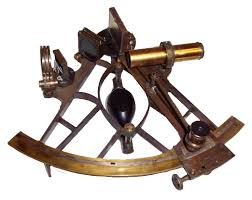
\includegraphics[width=10cm]{papers/nav/bilder/sextant.jpg}
	\caption[Sextant]{Sextant}
\end{figure}
\subsection{Bestimmung des eigenen Standortes $P$} \label{p}
Wir nehmen die Abbildung \ref{d2} zur Hilfe.
Nun hat man die Koordinaten der beiden Gestirne und man weiss die Koordinaten des Nordpols.
Damit wir unseren Standort bestimmen können, bilden wir zuerst das Dreieck $ABC$, dann das Dreieck $BPC$ und zum Schluss noch das Dreieck $ABP$.
Auf diese Dreiecke können wir die einfachen Sätze der sphärischen Trigonometrie anwenden und benötigen lediglich ein Ephemeride zu den Gestirnen und einen Sextant.

\begin{figure}
\centering
	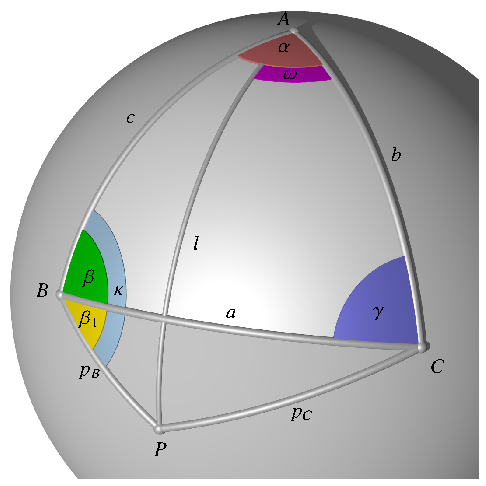
\includegraphics[width=8cm]{papers/nav/images/dreieck3d8.pdf}
	\caption[Dreieck für die Standortbestimmung]{Dreieck für die Standortbestimmung}
	\label{d2}
\end{figure}

\subsubsection{Dreieck $ABC$}

\begin{center}
	\begin{tabular}{ l l l }
		Ecke && Name  \\ 
		\hline
		$A$ && Nordpol \\  
		$B$ && Bildpunkt des Gestirns $X$ \\
		$C$&& Bildpunkt des Gestirns $Y$
	\end{tabular}
\end{center}

Mit unserem erlangten Wissen können wir nun alle Seiten des Dreiecks $ABC$ berechnen.
Dazu sind die folgenden vorbereitenden Berechnungen nötig:
\begin{enumerate}
	\item Die Seite vom Nordpol zum Bildpunkt $X$ sei $c$, dann ist $c = \frac{\pi}{2} - \delta_1$.  
	\item Die Seite vom Nordpol zum Bildpunkt $Y$ sei $b$, dann ist $b = \frac{\pi}{2} - \delta_2$.
	\item Der Innenwinkel bei der Ecke, wo der Nordpol ist sei $\alpha$, dann ist $ \alpha = |\lambda_1 - \lambda_2|$.
\end{enumerate}
mit 
\begin{center}
	\begin{tabular}{ l l l }
		Ecke && Name  \\ 
		\hline
		$\delta_1$ && Deklination vom Bildpunkt $X$ \\  
		$\delta_2$ && Deklination vom Bildpunk $Y$ \\
		$\lambda_1 $&& Längengrad vom Bildpunkt $X$\\
		$\lambda_2$ && Längengrad vom Bildpunkt $Y$
	\end{tabular}
\end{center}

Nun haben wir die beiden Seiten $c$ und $b$ und den Winkel $\alpha$, der sich zwischen diesen Seiten befindet. 
Mithilfe des Seiten-Kosinussatzes 
$\cos(a) = \cos(b)\cdot \cos(c) + \sin(b) \cdot \sin(c)\cdot \cos(\alpha)$ 
können wir nun die dritte Seitenlänge bestimmen. 
Es ist darauf zu achten, dass hier natürlich die Seitenlängen in Bogenmass sind und dementsprechend der Kosinus und Sinus verwendet wird. 

Jetzt fehlen noch die beiden anderen Innenwinkel $\beta$ und\ $\gamma$.
Diese bestimmen wir mithilfe des Kosinussatzes:
\[
\beta=\cos^{-1}  \bigg[\frac{\cos(b)-\cos(a) \cdot \cos(c)}{\sin(a) \cdot \sin(c)}\bigg]
\]
und
\[
\gamma =  \cos^{-1}  \bigg[\frac{\cos(c)-\cos(b) \cdot \cos(a)}{\sin(a) \cdot \sin(b)}\bigg]
\].

Schlussendlich haben wir die Seiten $a$, $b$ und $c$, die Ecken $A$,$B$ und $C$ und die Winkel $\alpha$, $\beta$  und  $\gamma$ bestimmt und somit das ganze Kugeldreieck $ABC$ berechnet.

\subsubsection{Dreieck $BPC$}
Wir bilden nun ein zweites Dreieck, welches die Ecken $B$ und $C$ des ersten Dreiecks besitzt. 
Die dritte Ecke ist der eigene Standort $P$.
Unser Standort definiere sich aus einer geographischen Breite
$\delta$ und einer geographischen Länge $\lambda$.

Die Seite von $P$ zu $B$ sei $p_B$ und die Seite von $P$ zu $C$ sei $p_C$.
Die beiden Seitenlängen kann man mit dem Sextant messen und durch eine einfache Formel bestimmen, nämlich $p_B=\frac{\pi}{2} - h_{B}$ und $p_C=\frac{\pi}{2} - h_{C}$ 
mit $h_B=$ Höhe von Gestirn in $B$ und $h_C=$ Höhe von Gestirn in $C$ mit Sextant gemessen.

Zum Schluss müssen wir noch den Winkel $\beta_1$ mithilfe des Seiten-Kosinussatzes
\[
\cos(p_B)=\cos(p_C)\cdot\cos(a)+\sin(p_C)\cdot\sin(a)\cdot\cos(\beta_1)
\]
mit den bekannten Seiten $p_C$, $p_B$ und $a$ bestimmen. 
\subsubsection{Dreieck $ABP$}
Nun muss man eine Verbindungslinie des Standorts zwischen $P$ und $A$ ziehen.
Die Länge $l$ dieser Linie entspricht der gesuchten geographischen Breite $\delta$.
Diese lässt sich mithilfe des Dreiecks $ABP$, den bekannten Seiten $c$ und $p_B$ und des Seiten-Kosinussatzes berechnen.
Für den Seiten-Kosinussatz benötigt es noch $\kappa=\beta + \beta_1$.
Somit ist
\[
\cos(l) = \cos(c)\cdot \cos(p_B) + \sin(c) \cdot \sin(p_B) \cdot \cos(\kappa)
\]
und
\[
\delta  =\cos^{-1} [\cos(c) \cdot \cos(p_B) + \sin(c) \cdot \sin(p_B) \cdot \cos(\kappa)].
\]

Für die geographische Länge $\lambda$ des eigenen Standortes nutzt man den Winkel $\omega$, welcher sich im Dreieck $ACP$ in der Ecke bei $A$ befindet.
Mithilfe des Kosinussatzes können wir
\[
\omega = \cos^{-1}  \bigg[\frac{\cos(p_B)-\cos(c) \cdot \cos(l)}{\sin(c) \cdot \sin(l)}\bigg]
\]
berechnen und bekommen schlussendlich die geographische Länge 
\[
\lambda=\lambda_1 - \omega,
\]
wobei $\lambda_1$ die Länge des Bildpunktes $X$ von $C$ ist.
